\section{The transcriptional landscape of \cer{}} %check again this stuff. i'm not convinced

The rise of microarrays and next generation sequencing techniques has made the exploration of the transcriptome possible. 
Early application of tiling arrays to the transcriptome of \cer{} showed that the genome is pervasively transcribed and RNA molecules can arise from almost any place \cite{neil:2009:widespread,xu:2009:bidirectional}. 
There are multiple reasons for this phenomenon.
Chief among all is the fact that the genome provides a very low barrier to transcription initiation.
Removing or displacing nucleosomes is often enough to allow basal levels of transcription to initiate, even without any of the regulatory sequences usually found at promoters.
Secondarily, studies have shown that yeast promoters do not posses an inherent direction dictated by sequence elements, but are bidirectional \cite{neil:2009:widespread,xu:2009:bidirectional}.

Promoter bidirectionality, and the general propensity of transcription to initiate spuriously, contribute to the generation of large quantities of non-functional RNAs, usually referred to as pervasive transcripts.
In order to prevent these RNAs from interfering with physiological activities, the cell evolved strict RNA quality control systems, active both in the nucleus and in the cytoplasm.
The vast majority of pervasive transcripts are subjected to quality control, and are degraded shortly after their production.

\subsection{RNA quality control systems}
\glsreset{nmd}

RNA quality control eliminates aberrant and pervasive transcripts through degradation.
Several multisubunit complexes located throughout the cell carry out this function through use of endo- and exo-nuclease activities.
Targeting of transcripts to these complexes (i.e. marking for degradation) can occur through several means: it can be directly connected to the termination mechanism used to release the transcript (as in the case of \gls{nns} termination), or it can depend on certain features of the RNA, such as lack of 5' cap or presence of a premature stop codon.
This ensures that pervasive and aberrant transcripts are extensively degraded both in the nucleus and in the cytoplasm.

The exosome is known to act in both these cellular compartments.
Its catalytic activity depends on the subunit Dis3\footnote{additional details on the structure of the exosome and \gls{tramp} are presented in section \ref{secTramp}}, that possesses \TtoF{} exonuclease and endonuclease activity.
In the nucleus, the exosome is associated with two specific co-factors: a second \TtoF{} exonuclease called Rrp6, and a polyadenylation complex called \gls{tramp}.
While Rrp6 significantly contributes to RNA degradation through its exonuclease activity, \gls{tramp} stimulates the activity of the exosome through addition of short poly(A) tails (and possibly other, less clear means).
This ensemble of interactions make the exosome the foremost quality control agent in the nucleus.
In the cytoplasm, the exosome is not found in complex with Rrp6 or \gls{tramp} and has only a minor role in RNA degradation.

In the cytoplasm, RNA quality control is mainly enforced by the \FtoT{} exonuclease Xrn1.
Several decay pathways can lead to degradation by Xrn1 (and to some extent the cytoplasmic exosome): \gls{nmd}, triggered by presence of a premature stop codon; \gls{ngd}, triggered by lack of a start codon; and \gls{nsd}, caused by lack of a stop codon.
The ensemble of these pathways targets transcripts that do not possess the typical features of mRNAs, stopping potentially toxic elements from being translated.
Xrn1 is known to target pervasive transcripts with poor coding potential in the cytoplasm, providing a backup system that can deal with those RNAs that manage to escape the nuclear quality control.

Recently, an additional role in quality control has been proposed for the \FtoT{} exonuclease Rat1 \cite{jimenogonza:2010:yeast}. 
Rat1 is one of the main actor of the torpedo model for \gls{cpf} termination and is thought to mediate the disassembly of the elongation complex once the transcript has been cleaved.
Using \gls{pol2} mutants unable to mediate capping of the transcript, the authors observed that Rat1-dependent transcription termination was occurring upstream of the cleavage site.
Rat1 was therefore implicated in degrading and prematurely terminating transcripts that could not be properly capped.
This would happen through a torpedo-like mechanism, thanks to the free 5'-P that provides an attack substrate for Rat1.

\subsection{Types of pervasive transcripts}

Because of the rapid turnover dictated by quality control systems, pervasive transcripts are extremely difficult to detect in wild type cells.
Several studies found that knocking-out certain elements of RNA quality control would affect the stability of some RNAs, making them appear in transcriptome analyses.
Over time, it became obvious that several classes of pervasive transcripts existed, each responding differently to inactivation of specific quality control pathways.
These classes, therefore, represent sets of transcripts sharing one or more features which make them more or less susceptible to specific branches of quality control.

\begin{figure}[ht]

\centering
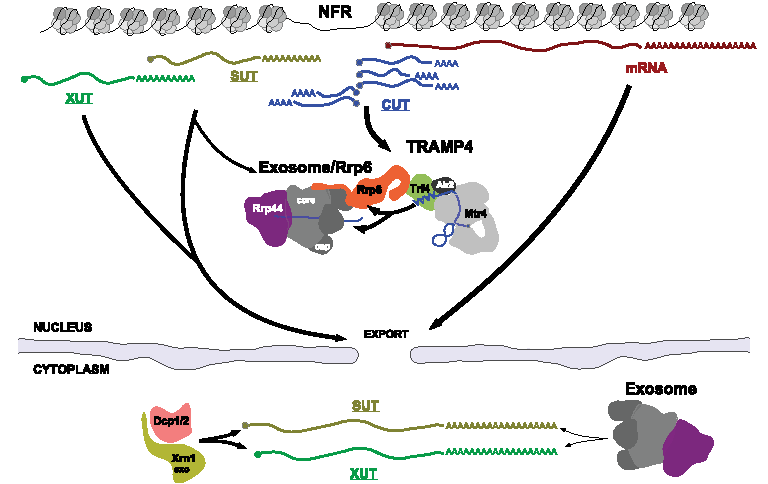
\includegraphics[width=\textwidth]{figures/introduction/pervasiveTr}
\caption[Classes of transcripts and their fates.]{The cellular fate of pervasive transcripts. Different classes of non-coding RNAs are represented at the top. Black arrows indicate the fate of the transcript after transcription, either immediate degradation via the exosome/\gls{tramp} quality control pathway, or export to the cytoplasm. Here, cytoplasmic quality control is shown.}
\label{fig:nnsTermination}

\end{figure}

\paragraph{CUTs}

The first---and most abundant---class of pervasive transcripts to be described, \gls{cuts} emerged from the deletion of the nuclear exosome co-factor Rrp6 \cite{wyers:2005:cryptic}.
\gls{cuts} are short transcripts (600-800 bp) originating from intergenic regions and bidirectional promoters.
They can often be detected in the antisense direction to protein-coding genes and their transcription can sometimes contribute to gene regulation.
\gls{cuts} are terminated by the \gls{nns} pathway.
This greatly facilitates their turnover, which happens exclusively in the nucleus.
After transcription termination has occurred, \gls{cuts} are contacted by \gls{tramp} and handed over to the nuclear exosome, resulting in their rapid degradation. \TODO{refs to termination of cuts by nns.}

\paragraph{SUTs}

Unlike \gls{cuts}, \gls{suts} are detectable in wild type cells \cite{david:2006:highresolution}.
This difference is due to the different termination mechanism that characterizes these transcripts.
While \gls{cuts} are terminated early by the \gls{nns} pathway, \gls{suts} are longer and terminate through the \gls{cpf} pathway \cite{marquardt:2011:distinct}.
The difference in termination implies that \gls{suts} can more easily escape the nuclear quality control, although it should be noted that a large portion of \gls{suts} is partially affected by exosome mutations \cite{gudipati:2012:extensive, marquardt:2011:distinct}.
Despite being exported to the cytoplasm, \gls{suts} have poor coding potential and are targeted by the cytoplasmic quality control pathways and degraded by Xrn1 \cite{malabat:2015:quality}. 

\paragraph{XUTs}

Very close to \gls{suts}, \gls{xuts} have essentially the same characteristics.
They are terminated by the \gls{cpf} pathway and rapidly exported to the cytoplasm.
However, while the turnover rate of \gls{suts} is sufficiently slow to allow their detection in wild type cells, \gls{xuts} are more susceptible to cytoplasmic decay pathways and require deletion of Xrn1 to become visible in trascriptome analyses \cite{vandijk:2011:xuts}.
  
\paragraph{NUTs}

Largely overlapping with \gls{cuts}, \gls{nuts} are defined as transcripts that gain stability when \gls{nns} termination is impaired \cite{schulz:2013:transcriptome}.
Normally, these transcripts are rapidly degraded by the nuclear exosome.
However, when \gls{nns} termination is impaired, these transcript gain in length and stability, becoming detectable.


\paragraph{RUTs}

Only recently identified as a new class of pervasive transcripts \cite{colin:2014:roadblock}, \gls{ruts} are transcripts subjected to road-block termination by the transcription factor Reb1 and subsequently degraded by the nuclear exosome.

\subsection{Function of pervasive transcripts}

The question of whether pervasive transcripts in yeast possess any functional activity remains unclear.
While the act of pervasive transcription has been associated with regulatory events on multiple occasions, very little is known about the function of the transcripts themselves.
For example, SER3 expression is known to be  regulated by the upstream non-coding RNA SRG1 through a mechanism of transcriptional interference \cite{martens:2004:intergenic}.  
Similarly, the PHO84 gene seems to be regulated by an antisense transcript that runs along the whole gene, reaching the promoter and downregulating expression \cite{castelnuovo:2013:bimodal}.
In both these cases, repression is mediated through a modification of the chromatin state of the promoter, which prevents assembly of the \acrlong{pic}.
Stabilization of the transcript, however, did not in any way affect the repression.

Other regulation mechanisms involve \gls{nns} termination and a conditional generation of cuts.
Several nucleotide biosynthesis genes (URA2, URA8, IMD2 among others) can initiate transcription from two regions separated by an \gls{nns} terminator sequence.
Nucleotide availability can modify the \gls{tss} selection behaviour of \gls{pol2}, resulting in productive elongation only if the downstream \gls{tss} is selected.

%Pervasive transcription represents a concrete danger to cell viability.
%However, the cell has adapted several mechanisms to deal with its products, while limiting the impact of the transcription events themselves, or hijacking them for regulatory purposes.


\clearpage



